\documentclass{article}

\usepackage{graphicx}
\usepackage{subfigure}
\usepackage[hypcap]{caption}
\usepackage{listings}
\usepackage{float}
\floatstyle{plaintop}
\restylefloat{table}

\title{Experimental Design and Data Analysis: Assignment 4}
\author{Andrew Bedard(2566978) \& Simone van Gompel(2567525) \\ Group 19}

\begin{document}

  \maketitle

  \section*{Exercise 1}
    \subsection*{1}
    \subsection*{2}
    \subsection*{3}
    \subsection*{4}
    
  \section*{Exercise 2}
    \subsection*{1}
      \begin{figure}[H]
          \centering
          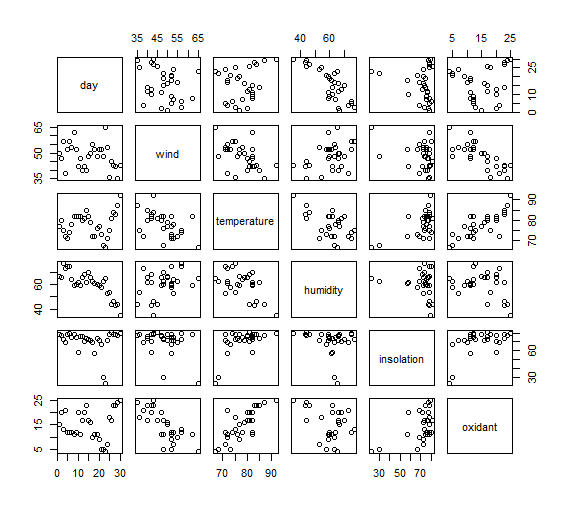
\includegraphics[scale=0.6]{../results/2_1.png}
          \caption{Pairplot of the airpollution data}
          \label{fig:BoxHours}
      \end{figure} 
    \subsection*{2}
      \begin{figure}[H]
          \centering
          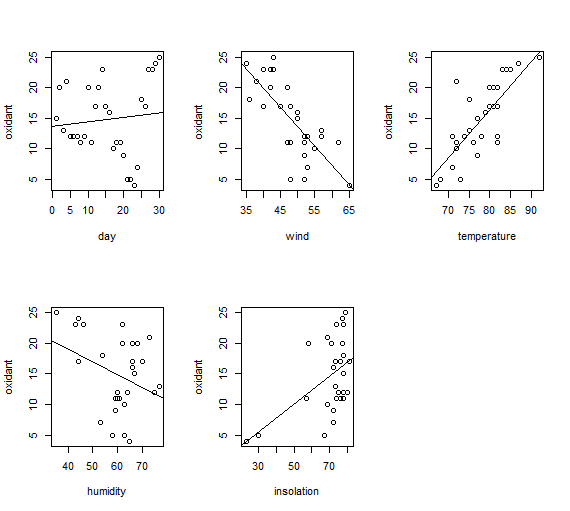
\includegraphics[scale=0.6]{../results/2_2.png}
          \caption{The linear regression of the explanatory variables}
          \label{fig:BoxHours}
      \end{figure} 
    \subsection*{3}
    \subsection*{4}
    \subsection*{5}

  \section*{Exercise 3}
    \subsection*{1}
    \subsection*{2}
    \subsection*{3}
    \subsection*{4}
    \subsection*{5}

  \section*{Exercise 4}
    Following the step-up method we get for the first variable:
    \begin{table}[H]
    \begin{center}
    \begin{tabular}{l|l}
        Variable & $R^2$ \\
        \hline 
        Expend\textasciitilde Pop & 0.9073 \\
        Expend\textasciitilde Employ & 0.954 \\
        Expend\textasciitilde Lawyers & 0.9373 \\
        Expend\textasciitilde Crime & 0.1119 \\
        Expend\textasciitilde Bad & 0.6964 \\
    \end{tabular}
    \caption{Results of 1-way Anova on square root of \textit{genal.txt} data}
    \label{table:step1}
    \end{center}
    \end{table}
    Expend\textasciitilde Employ had the highest score, so we take this for the second step:
    \begin{table}[H]
    \begin{center}
    \begin{tabular}{l|l}
        Variable & $R^2$ \\
        \hline 
        Expend\textasciitilde Employ+Pop & 0.9543 \\
        Expend\textasciitilde Employ+Lawyers & 0.9632 \\
        Expend\textasciitilde Employ+Crime & 0.9551 \\
        Expend\textasciitilde Employ+Bad & 0.9551 \\
    \end{tabular}
    \caption{Results of 1-way Anova on square root of \textit{genal.txt} data}
    \label{table:step2}
    \end{center}
    \end{table}
    Expend\textasciitilde Employ+Lawyer had the highest score, so we take this for the third step:
    \begin{table}[H]
    \begin{center}
    \begin{tabular}{l|l}
        Variable & $R^2$ \\
        \hline 
        Expend\textasciitilde Employ+Lawyers+Pop & 0.9637 \\
        Expend\textasciitilde Employ+Lawyers+Crime & 0.9632 \\
        Expend\textasciitilde Employ+Lawyers+Bad & 0.9639 \\
    \end{tabular}
    \caption{Results of 1-way Anova on square root of \textit{genal.txt} data}
    \label{table:step3}
    \end{center}
    \end{table}
    Adding these variables yield no significant change and so we stop at the second step.
    The result of Expend\textasciitilde Employ+Lawyer is:\\
    \begin{lstlisting}[language=R]
Coefficients:
              Estimate Std. Error t value Pr(>|t|)    
(Intercept) -1.107e+02  4.257e+01  -2.600  0.01236 *  
employ       2.971e-02  5.114e-03   5.810 4.89e-07 ***
lawyers      2.686e-02  7.757e-03   3.463  0.00113 ** 
Multiple R-squared:  0.9632
    \end{lstlisting}
    
  \section{R-Code}
    \subsection{Exercise 1}\label{sec:RE1}
      \begin{lstlisting}[language=R]
      \end{lstlisting}
    \subsection{Exercise 2}\label{sec:RE2}
      \begin{lstlisting}[language=R]
      \end{lstlisting}
    \subsection{Exercise 3}\label{sec:RE3}
      \begin{lstlisting}[language=R]
      \end{lstlisting}
    \subsection{Exercise 4}\label{sec:RE4}
      \begin{lstlisting}[language=R]
      \end{lstlisting}
\end{document}
